%%%%%%%%%%%%%%%%%%%%%%%%%%%%%%%%%%%%%%%%%%%%%%%%%%%%%%%%%%%%%%%%%%%%%%%%%%%%
%  第15回 例題5〜7（原本 20161215143926.pdf の p70/p72/p73 より）
%  原本は「問題枠 →(指針)空欄→【KEY】」で解答が載っていないため，
%  【指針】と【解答】は本文の説明・練習問題の解答の解き方に合わせて書き起こした．
%  ※ このファイルは記録用。実体は physics_ch15.tex に流し込み済み。
%%%%%%%%%%%%%%%%%%%%%%%%%%%%%%%%%%%%%%%%%%%%%%%%%%%%%%%%%%%%%%%%%%%%%%%%%%%%

%%%%%%%%%%%%%%%%%%%%  例題5（15.1 の直後）  %%%%%%%%%%%%%%%%%%%%
\begin{reidai}{気体分子運動論}
\begin{zuright}{42mm}
\hspace{1zw}気体分子の運動に関する以下の問に答えよ．ただし，速度，運動量，力積は$x$, $y$, $z$軸正の向きを正とする．\par
\hspace{1zw}一辺の長さが$l\U{m}$の立方体の容器があり，その中に$n\U{mol}$の理想気体が封入されている．気体分子1つあたりの質量を$m\U{kg}$とし，簡単のため分子同士が衝突することはないものと仮定する．\par
\hspace{1zw}今，気体分子の1つに着目し，この気体分子の持つ速度が$(v_x, v_y, v_z)\U{m/s}$だったとする．この分子が図に示した面に完全弾性衝突し，この気体分子の持つ速度が$(v_x', v_y', v_z')\U{m/s}$になったとする．
\zusep
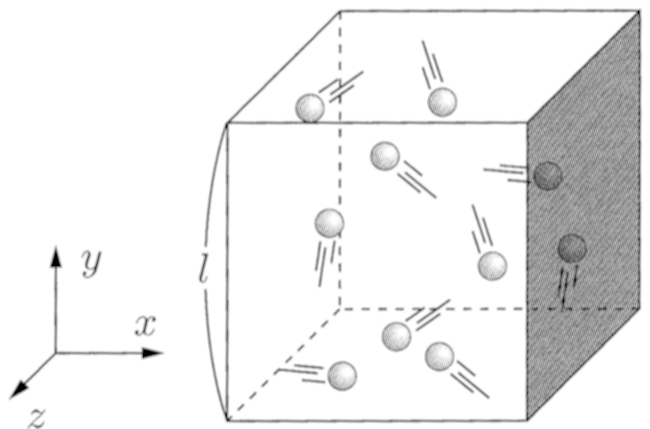
\includegraphics[keepaspectratio,width=42mm]{fig/ch15_ex5_cube.png}\\[3mm]
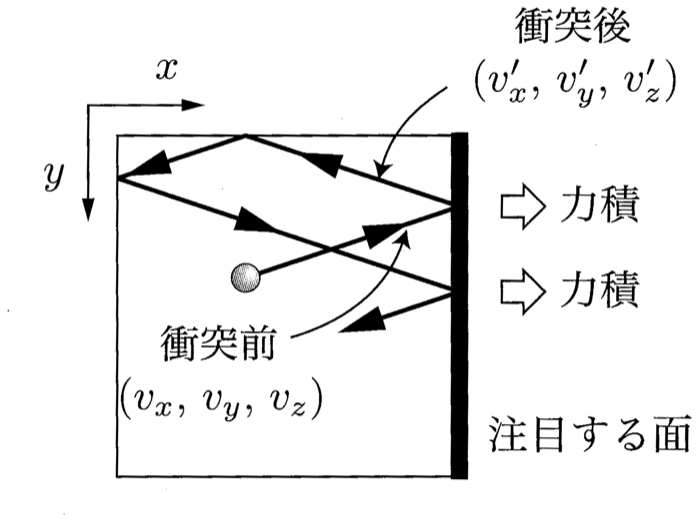
\includegraphics[keepaspectratio,width=42mm]{fig/ch15_ex5_hane.png}
\end{zuright}
\begin{komon}
\ko{1} 衝突後の速度$(v_x', v_y', v_z')$を$v_x$, $v_y$, $v_z$を用いて表せ．
\ko{2} 気体分子の持つ運動量の$x$軸方向成分の衝突1回あたりの変化$\Delta p\U{N\cdot s}$を求めよ．
\ko{3} 気体分子がこの1回の衝突により壁面に与えた力積の大きさを求めよ．
\end{komon}
\hspace{1zw}以上より，この気体分子が他の壁に衝突したとしても$x$軸方向の速度の大きさ$|v_x|\U{m/s}$は不変である．
\begin{komon}
\ko{4} この気体分子が図の面に衝突したのち再びこの面に衝突するまでにかかる時間$\tau\U{s}$を求めよ．
\ko{5} (4)を元に，この気体分子が時間$t\U{s}$の間に図の面に衝突する回数を求めよ．
\ko{6} 以上より，この気体分子が時間$t\U{s}$の間に図の面に与える力積の大きさを求めよ．
\end{komon}
\begin{zuright}{50mm}
\hspace{1zw}実際にはこの面に力（力積）が作用するのは不連続で，とぎれとぎれに作用しているが，実際には再衝突までの時間が短いために，あたかも一定の力が連続的に作用しているかのように感じられる．作用する時間を$t\U{s}$，作用する平均の力の大きさを$\overline{F}\U{N}$とする．
\zusep
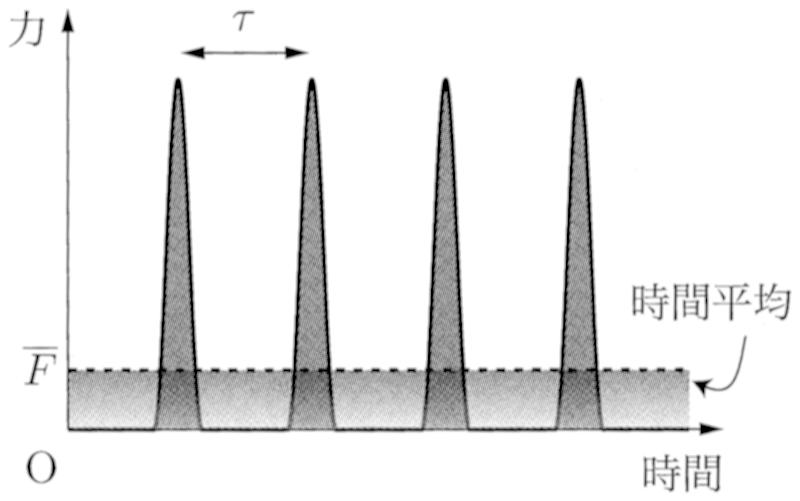
\includegraphics[keepaspectratio,width=50mm]{fig/ch15_ex5_Ft.png}
\end{zuright}
\begin{komon}
\ko{7} (6)より，この1分子が壁に作用する平均の力の大きさ$\overline{F}\U{N}$を求めよ．
\end{komon}
\hspace{1zw}さて，実際には分子ごとに分子の持つ速度は異なっている．よって分子ごとに$\overline{F}\U{N}$の値も異なるが，これを全分子に対して平均化することを考える．$x$軸方向の速度$v_x$の二乗の平均値を$\overline{v_x^2}$とおく．
\begin{komon}
\ko{8} 平均して1分子あたりがこの壁面に対して及ぼす力の大きさを求めよ．
\ko{9} 気体分子の運動は容器の形状によらずに空間に対して等方的である．このことから，$\overline{v_x^2}$, $\overline{v_y^2}$, $\overline{v_z^2}$の間に成り立つ関係式を示せ．
\ko{10} (9)より，(8)の1分子あたりの力を気体分子の持つ速度の大きさ$v\U{m/s}$の二乗平均$\overline{v^2}\U{m^2/s^2}$を用いて表せ．
\ko{11} アボガドロ数を$N_{\mathrm{A}}$として，この容器内に入っている気体分子の総数を求めよ．
\ko{12} これらより，壁に作用する全力の大きさ，および壁に作用する圧力$p\U{Pa}$を求めよ．
\ko{13} 容器の体積を$V(=l^3)\U{m^3}$とする．$pV$の値を求めよ．
\end{komon}
\hspace{1zw}理想気体であれば，気体定数$R\U{J/mol\cdot K}$，気体の温度$T\U{K}$を用いて状態方程式$pV=nRT$が成立する．
\begin{komon}
\ko{14} (13)と状態方程式を元に，気体分子の二乗平均平方根速度$\sqrt{\overline{v^2}}\U{m/s}$を，気体分子の$1\U{mol}$あたりの質量$M\U{kg/mol}$を用いて表せ．
\end{komon}
\end{reidai}

\begin{sisinE}
気体分子運動論の問題は，圧力を求めるまでの流れが決まっている．その道筋を把握しておくこと．本問はその流れを(1)から(13)まで順にたどるように作られている．

とくに混同しやすいのが「分子が受けた力積」と「分子が壁に与えた力積」，および「力積」と「力」である．前者は作用・反作用の法則で等大逆向き，後者は（力積）＝（平均の力）$\times$（作用した時間）で結ばれる．

(9)の等方性は，$x$, $y$, $z$のどの向きも同等であることから従う．三平方の定理$v^2=v_x^2+v_y^2+v_z^2$と合わせると$\overline{v_x^2}=\dfrac{1}{3}\overline{v^2}$となり，ここではじめて$\overline{v^2}$の式に書き換えられる．
\end{sisinE}

\begin{key}
\hspace{3mm} 衝突1回の力積\hspace{8mm} （運動量の変化）＝（分子が受けた力積）\\
\hspace{3mm} 作用・反作用\hspace{12mm} （分子が壁に与えた力積）＝$-$（壁が分子に与えた力積）\\
\hspace{3mm} 力積と平均の力\hspace{6mm} $\overline{F}\cdot t=$（時間$t\U{s}$の間に与えた力積の総和）\\
\hspace{3mm} 等方性\hspace{20mm} $\overline{v_x^2}=\overline{v_y^2}=\overline{v_z^2}=\dfrac{1}{3}\overline{v^2}$
\end{key}

\begin{kaitou}
\begin{komon}
\ko{1} 図の面は$x$軸に垂直であるから，完全弾性衝突では面に平行な$y$, $z$成分は変化せず，面に垂直な$x$成分だけが符号を変える．よって，
       \[(v_x', v_y', v_z')=(-v_x, v_y, v_z)\Ans\]
\ko{2} 運動量の$x$成分の変化は，
       \[\Delta p=mv_x'-mv_x=-2mv_x\U{N\cdot s}\Ans\]
\ko{3} (2)は分子が壁から受けた力積である．作用・反作用の法則より，分子が壁に与えた力積はこれと等大逆向きの$2mv_x\U{N\cdot s}$であるから，その大きさは
       \[2m|v_x|\U{N\cdot s}\Ans\]
\ko{4} 図の面に再び衝突するには，分子は$x$軸方向に往復分の$2l\U{m}$を進まなければならない．$x$軸方向の速さは$|v_x|$のまま変化しないので，
       \[\tau=\frac{2l}{|v_x|}\U{s}\Ans\]
\ko{5} 衝突の時間間隔は$\tau$で一定であるから，時間$t\U{s}$の間の衝突回数は
       \[\frac{t}{\tau}=\frac{|v_x|t}{2l}\,[\text{回}]\Ans\]
\ko{6} 1回あたり$2m|v_x|\U{N\cdot s}$を$\dfrac{|v_x|t}{2l}$回与えるから，
       \[2m|v_x|\cdot\frac{|v_x|t}{2l}=\frac{mv_x^2t}{l}\U{N\cdot s}\Ans\]
\ko{7} （力積）＝（平均の力）$\times$（作用した時間）より$\overline{F}\cdot t=\dfrac{mv_x^2t}{l}$であるから，
       \[\overline{F}=\frac{mv_x^2}{l}\U{N}\Ans\]
\ko{8} (7)の$v_x^2$を全分子について平均すればよいから，
       \[\overline{F}=\frac{m\overline{v_x^2}}{l}\U{N}\Ans\]
\ko{9} $x$, $y$, $z$のどの向きも同等であるから，
       \[\overline{v_x^2}=\overline{v_y^2}=\overline{v_z^2}\Ans\]
\ko{10} 三平方の定理$v^2=v_x^2+v_y^2+v_z^2$の両辺を全分子で平均すると$\overline{v^2}=\overline{v_x^2}+\overline{v_y^2}+\overline{v_z^2}$となり，(9)よりこれは$3\overline{v_x^2}$に等しい．よって$\overline{v_x^2}=\dfrac{1}{3}\overline{v^2}$であるから，
       \[\overline{F}=\frac{m\overline{v^2}}{3l}\U{N}\Ans\]
\ko{11} $n\U{mol}$あるから，分子の総数は
       \[N=nN_{\mathrm{A}}\,[\text{個}]\Ans\]
\ko{12} 壁に作用する全力の大きさは，(10)を全分子分足し合わせて
       \[N\overline{F}=\frac{nN_{\mathrm{A}}m\overline{v^2}}{3l}\U{N}\Ans\]
       壁の面積は$l^2\U{m^2}$であるから，圧力は
       \[p=\frac{nN_{\mathrm{A}}m\overline{v^2}}{3l\cdot l^2}=\frac{nN_{\mathrm{A}}m\overline{v^2}}{3l^3}\U{Pa}\Ans\]
\ko{13} $V=l^3$であるから，
       \[pV=\frac{nN_{\mathrm{A}}m\overline{v^2}}{3}\left(=\frac{Nm\overline{v^2}}{3}\right)\Ans\]
       これがベルヌーイの式である．
\ko{14} (13)と$pV=nRT$を結ぶと，
       \[\frac{nN_{\mathrm{A}}m\overline{v^2}}{3}=nRT\]
       ここで$M=mN_{\mathrm{A}}\U{kg/mol}$であるから，$\dfrac{M\overline{v^2}}{3}=RT$，すなわち$\overline{v^2}=\dfrac{3RT}{M}$となる．よって，
       \[\sqrt{\overline{v^2}}=\sqrt{\frac{3RT}{M}}\U{m/s}\Ans\]
\end{komon}
\end{kaitou}

%%%%%%%%%%  例題6（15.2 の直後）  %%%%%%%%%%%%%%%%%%%%
\begin{reidai}{単原子分子理想気体の内部エネルギー}
\begin{zuright}{50mm}
\hspace{1zw}容積が$V_1$, $V_2\U{m^3}$の断熱容器$\mathrm{A}$, $\mathrm{B}$をコック$\mathrm{K}$のついた細管でつなぐ．$\mathrm{K}$を閉じた状態で単原子分子理想気体を$\mathrm{A}$には圧力$P_1\U{Pa}$，温度$T_1\U{K}$で，$\mathrm{B}$には圧力$P_2\U{Pa}$，温度$T_2\U{K}$でそれぞれ注入した．$\mathrm{K}$を開いて十分時間を経過させるときの変化について，気体定数を$R\U{J/mol\cdot K}$として以下の問に答えよ．
\zusep
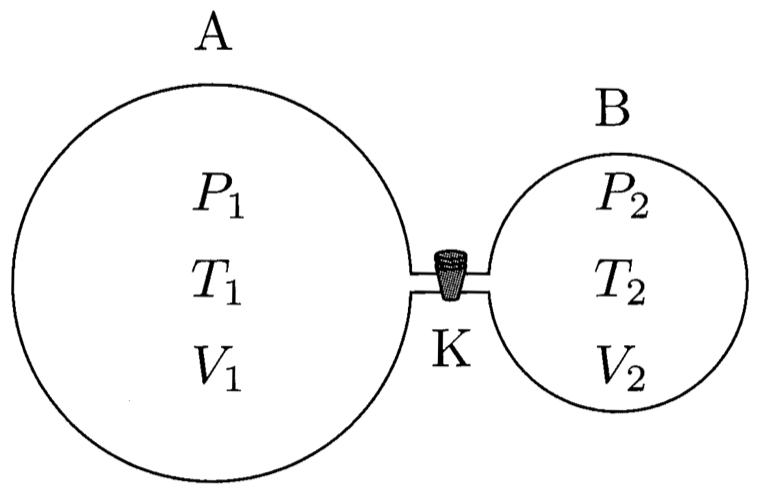
\includegraphics[keepaspectratio,width=50mm]{fig/ch15_ex6_cock.png}
\end{zuright}
\vspace{-\medskipamount}
\begin{komon}
\ko{1} $\mathrm{K}$を開く前に$\mathrm{A}$，$\mathrm{B}$に入っていた気体のモル数$n_1$, $n_2\U{mol}$を求めよ．
\ko{2} この状態変化で気体の内部エネルギーの総和は保存される．このことを利用して十分時間が経過した後の気体の温度$T\U{K}$を求めよ．
\ko{3} 十分時間が経過した後の容器内の気体の圧力$P\U{Pa}$を求めよ．
\end{komon}
\end{reidai}

\begin{sisinE}
容器は断熱されているので外界と熱のやり取りをせず（$Q=0$），容器全体の体積も変わらないので気体は仕事もしない（$W=0$）．よって熱力学第一法則より内部エネルギーの総和は変化しない，というのが(2)の「保存される」の中身である．

あとは単原子分子理想気体の内部エネルギーが$U=\dfrac{3}{2}nRT$と書けることを使えばよい．$nRT=PV$であることに注意すると，$U=\dfrac{3}{2}PV$と書き直せて計算がかなり楽になる．
\end{sisinE}

\begin{key}
\hspace{3mm} 単原子分子理想気体\hspace{4mm} $\Rightarrow$\hspace{4mm} 内部エネルギー$U=\dfrac{3}{2}nRT$
\end{key}

\begin{kaitou}
\begin{komon}
\ko{1} それぞれの状態方程式$P_1V_1=n_1RT_1$, $P_2V_2=n_2RT_2$より，
       \[n_1=\frac{P_1V_1}{RT_1}\U{mol},\quad n_2=\frac{P_2V_2}{RT_2}\U{mol}\Ans\]
\ko{2} 単原子分子理想気体であるから，$\mathrm{K}$を開く前の内部エネルギーの総和は，$nRT=PV$を用いて
       \[U=\frac{3}{2}n_1RT_1+\frac{3}{2}n_2RT_2=\frac{3}{2}(P_1V_1+P_2V_2)\]
       である．$\mathrm{K}$を開いた後は全体が温度$T\U{K}$の一様な状態になるから，そのときの内部エネルギーは
       \[U'=\frac{3}{2}(n_1+n_2)RT\]
       である．内部エネルギーの総和は保存されるので$U'=U$，すなわち
       \[(n_1+n_2)RT=P_1V_1+P_2V_2\]
       これに(1)を代入して，
       \[\left(\frac{P_1V_1}{T_1}+\frac{P_2V_2}{T_2}\right)T=P_1V_1+P_2V_2\]
       よって，
       \[T=\frac{T_1T_2(P_1V_1+P_2V_2)}{P_1V_1T_2+P_2V_2T_1}\U{K}\Ans\]
\ko{3} 十分時間が経過した後の気体は，体積$V_1+V_2\U{m^3}$，物質量$n_1+n_2\U{mol}$，温度$T\U{K}$であるから，状態方程式は
       \[P(V_1+V_2)=(n_1+n_2)RT\]
       である．(2)で得た$(n_1+n_2)RT=P_1V_1+P_2V_2$を代入して，
       \[P=\frac{P_1V_1+P_2V_2}{V_1+V_2}\U{Pa}\Ans\]
\end{komon}
\end{kaitou}

%%%%%%%%%%  例題7（15.3 の直後）  %%%%%%%%%%%%%%%%%%%%
\begin{reidai}{$P-V$図}
\begin{zuright}{44mm}
\hspace{1zw}一定量の理想気体の状態を図の矢印の順に静かに変化させた．$\mathrm{A}$での体積が$V_0\U{m^3}$であるときについて，この状態変化を$P-V$図上での変化に書き直せ．ただし，グラフには$\mathrm{A}$, $\mathrm{B}$, $\mathrm{C}$, $\mathrm{D}$点を明示し，変化の方向に矢印をつけること．
\zusep
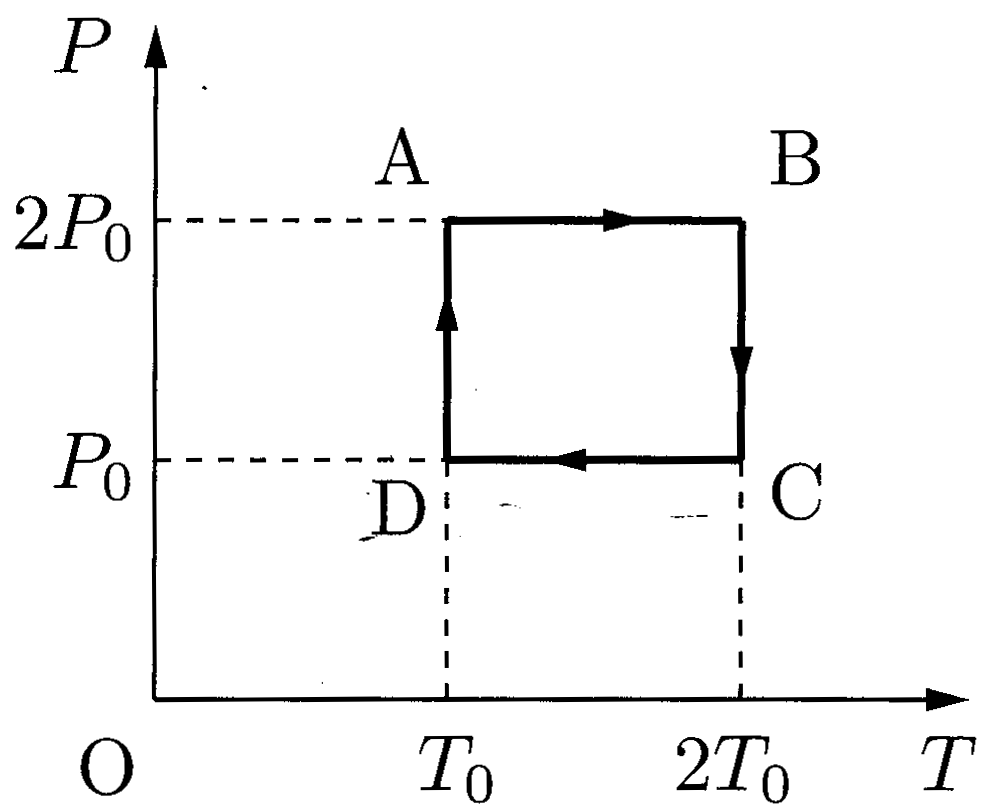
\includegraphics[keepaspectratio,width=44mm]{fig/ch15_ex7_pt.png}
\end{zuright}
\end{reidai}

\begin{sisinE}
例えば温度が変化しないならば，$pV=nRT$, $p'V'=nRT$のかわりに$pV=p'V'$を考えるなど，変化しない状態量を状態方程式から除いて考えると楽である．

まず4点それぞれの体積を状態方程式から求めて位置を決め，そのあとで各変化が定圧変化・等温変化のどちらであるかを見て，直線で結ぶか双曲線で結ぶかを決めればよい．
\end{sisinE}

\begin{kaitou}
\hspace{1zw}気体の物質量を$n\U{mol}$，気体定数を$R\U{J/mol\cdot K}$とする．与えられた図より，各点の圧力と温度は
\[\mathrm{A}(T_0,\,2P_0),\quad \mathrm{B}(2T_0,\,2P_0),\]
\[\mathrm{C}(2T_0,\,P_0),\quad \mathrm{D}(T_0,\,P_0)\]
である．$\mathrm{A}$での体積が$V_0$であるから，$\mathrm{A}$での状態方程式より
\[2P_0V_0=nRT_0\qquad \text{すなわち}\quad nR=\frac{2P_0V_0}{T_0}\]
となる．これを用いて各点の体積を求めると，
\[\mathrm{B}:2P_0V_{\mathrm{B}}=nR\cdot 2T_0\ \ \text{より}\ \ V_{\mathrm{B}}=2V_0\]
\[\mathrm{C}:P_0V_{\mathrm{C}}=nR\cdot 2T_0\ \ \text{より}\ \ V_{\mathrm{C}}=4V_0\]
\[\mathrm{D}:P_0V_{\mathrm{D}}=nR\cdot T_0\ \ \text{より}\ \ V_{\mathrm{D}}=2V_0\]
となる．\par
\hspace{1zw}次に各変化を見る．
\begin{komon}
\ko{1} $\mathrm{A}\to\mathrm{B}$は圧力が$2P_0$のまま変化しないので{\bf 定圧変化}であり，$P-V$図上では$P=2P_0$の水平な直線上を$V=V_0\to 2V_0$まで変化する．
\ko{2} $\mathrm{B}\to\mathrm{C}$は温度が$2T_0$のまま変化しないので{\bf 等温変化}であり，$PV=nR\cdot 2T_0=4P_0V_0$（一定）となる．すなわち$P-V$図上では双曲線$P=\dfrac{4P_0V_0}{V}$の上を$V=2V_0\to 4V_0$まで変化する．
\ko{3} $\mathrm{C}\to\mathrm{D}$は圧力が$P_0$のまま変化しないので{\bf 定圧変化}であり，$P=P_0$の水平な直線上を$V=4V_0\to 2V_0$まで変化する．
\ko{4} $\mathrm{D}\to\mathrm{A}$は温度が$T_0$のまま変化しないので{\bf 等温変化}であり，$PV=nRT_0=2P_0V_0$（一定）となる．すなわち双曲線$P=\dfrac{2P_0V_0}{V}$の上を$V=2V_0\to V_0$まで変化する．
\end{komon}
\hspace{1zw}以上をまとめると，求める$P-V$図は次のようになる．
\begin{center}
% 穴埋め版（生徒用）では答のグラフを軸だけの図に差し替える．
% 2枚は同じ画素寸法なので，貼付幅が同じなら両版のページ送りは揃う．
\ifbsAnaume
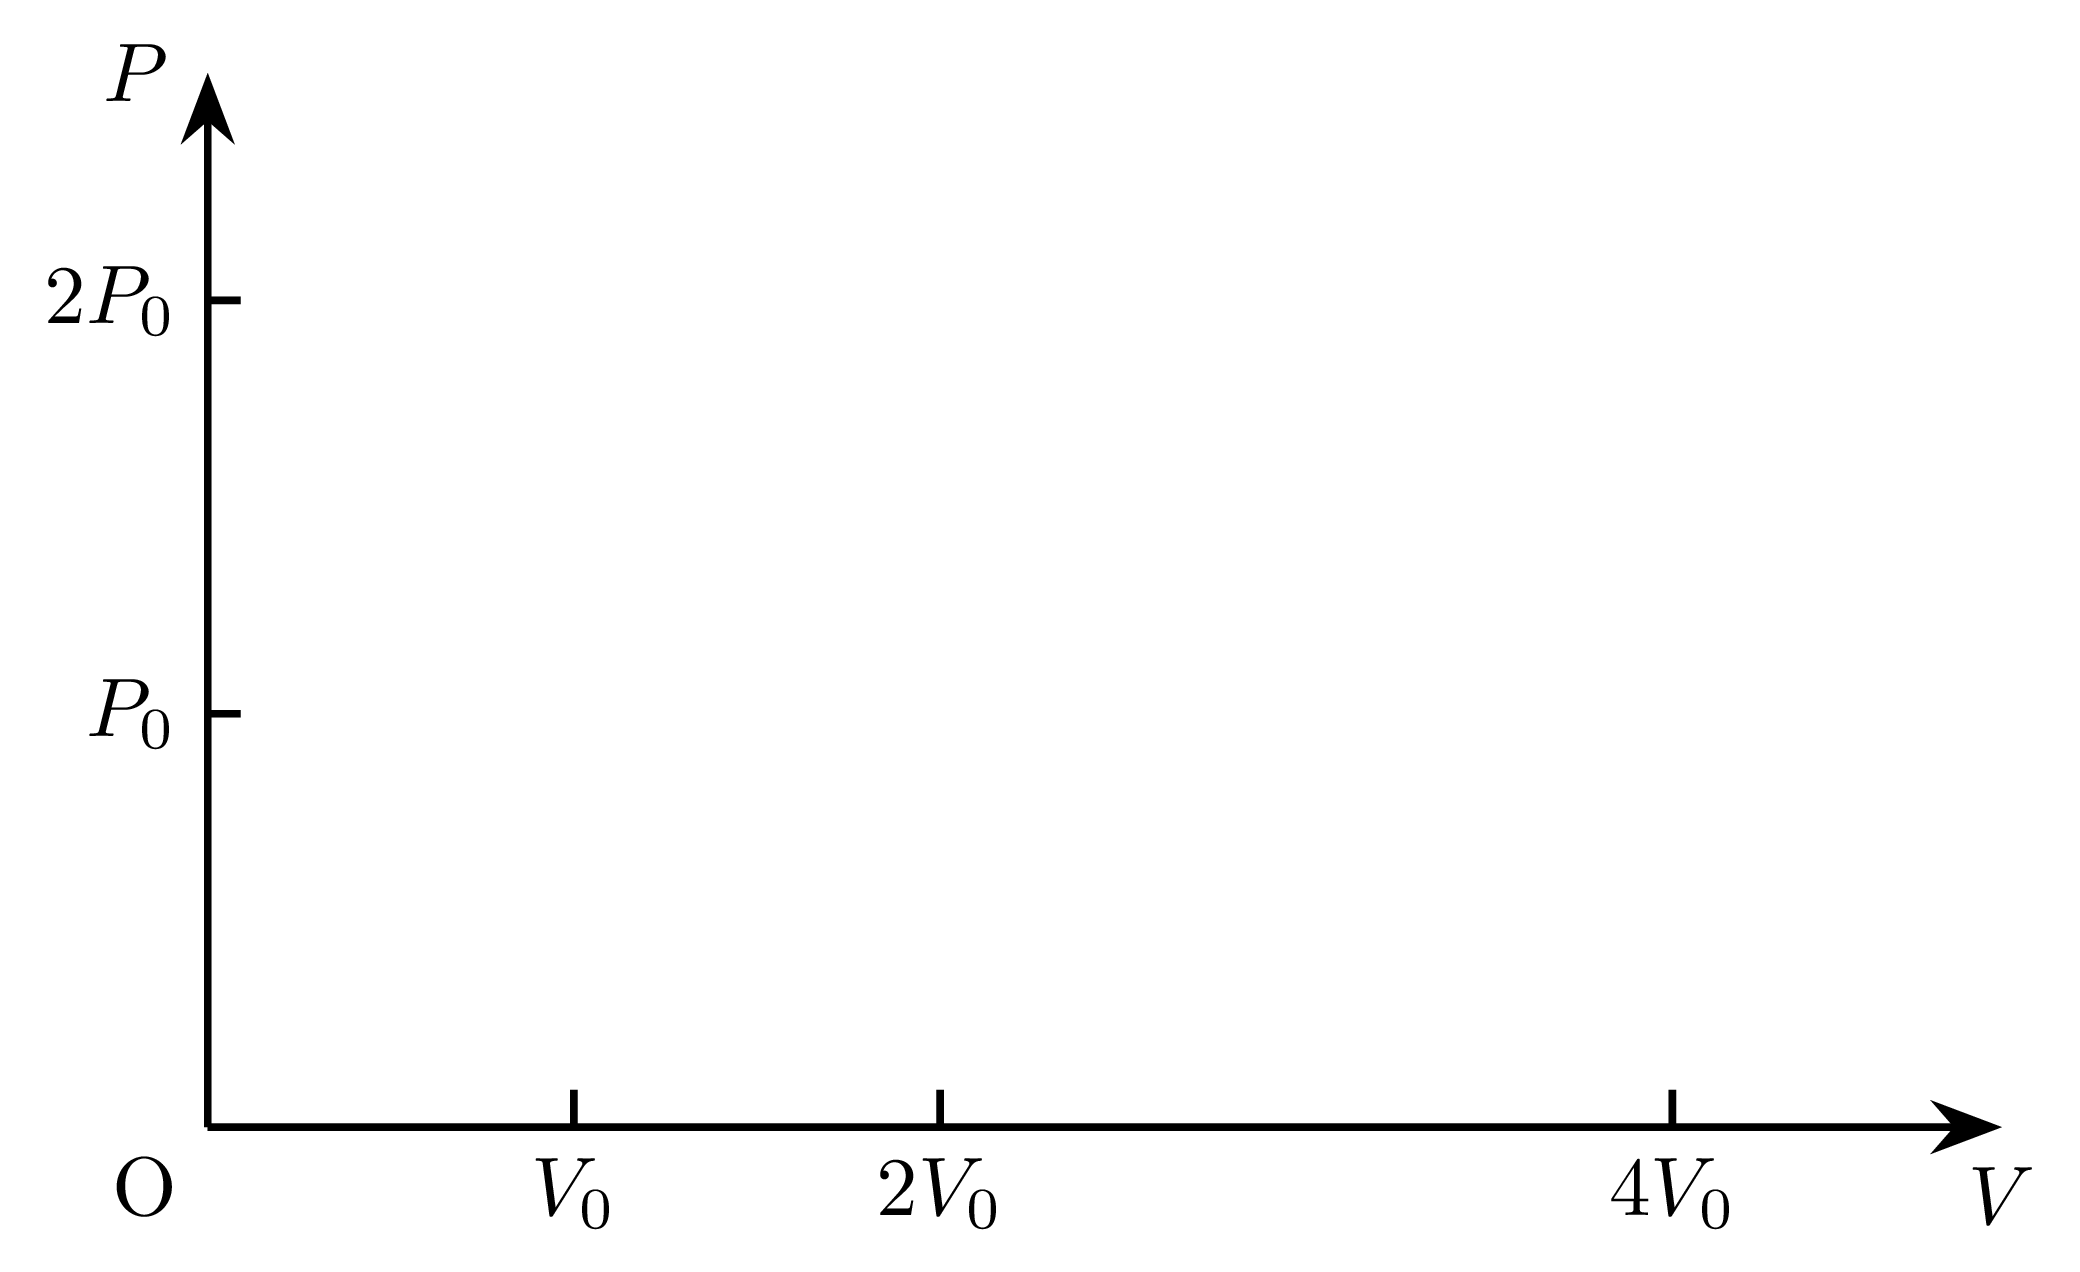
\includegraphics[keepaspectratio,width=76mm]{fig/ch15_ex7_pv_blank.png}
\else
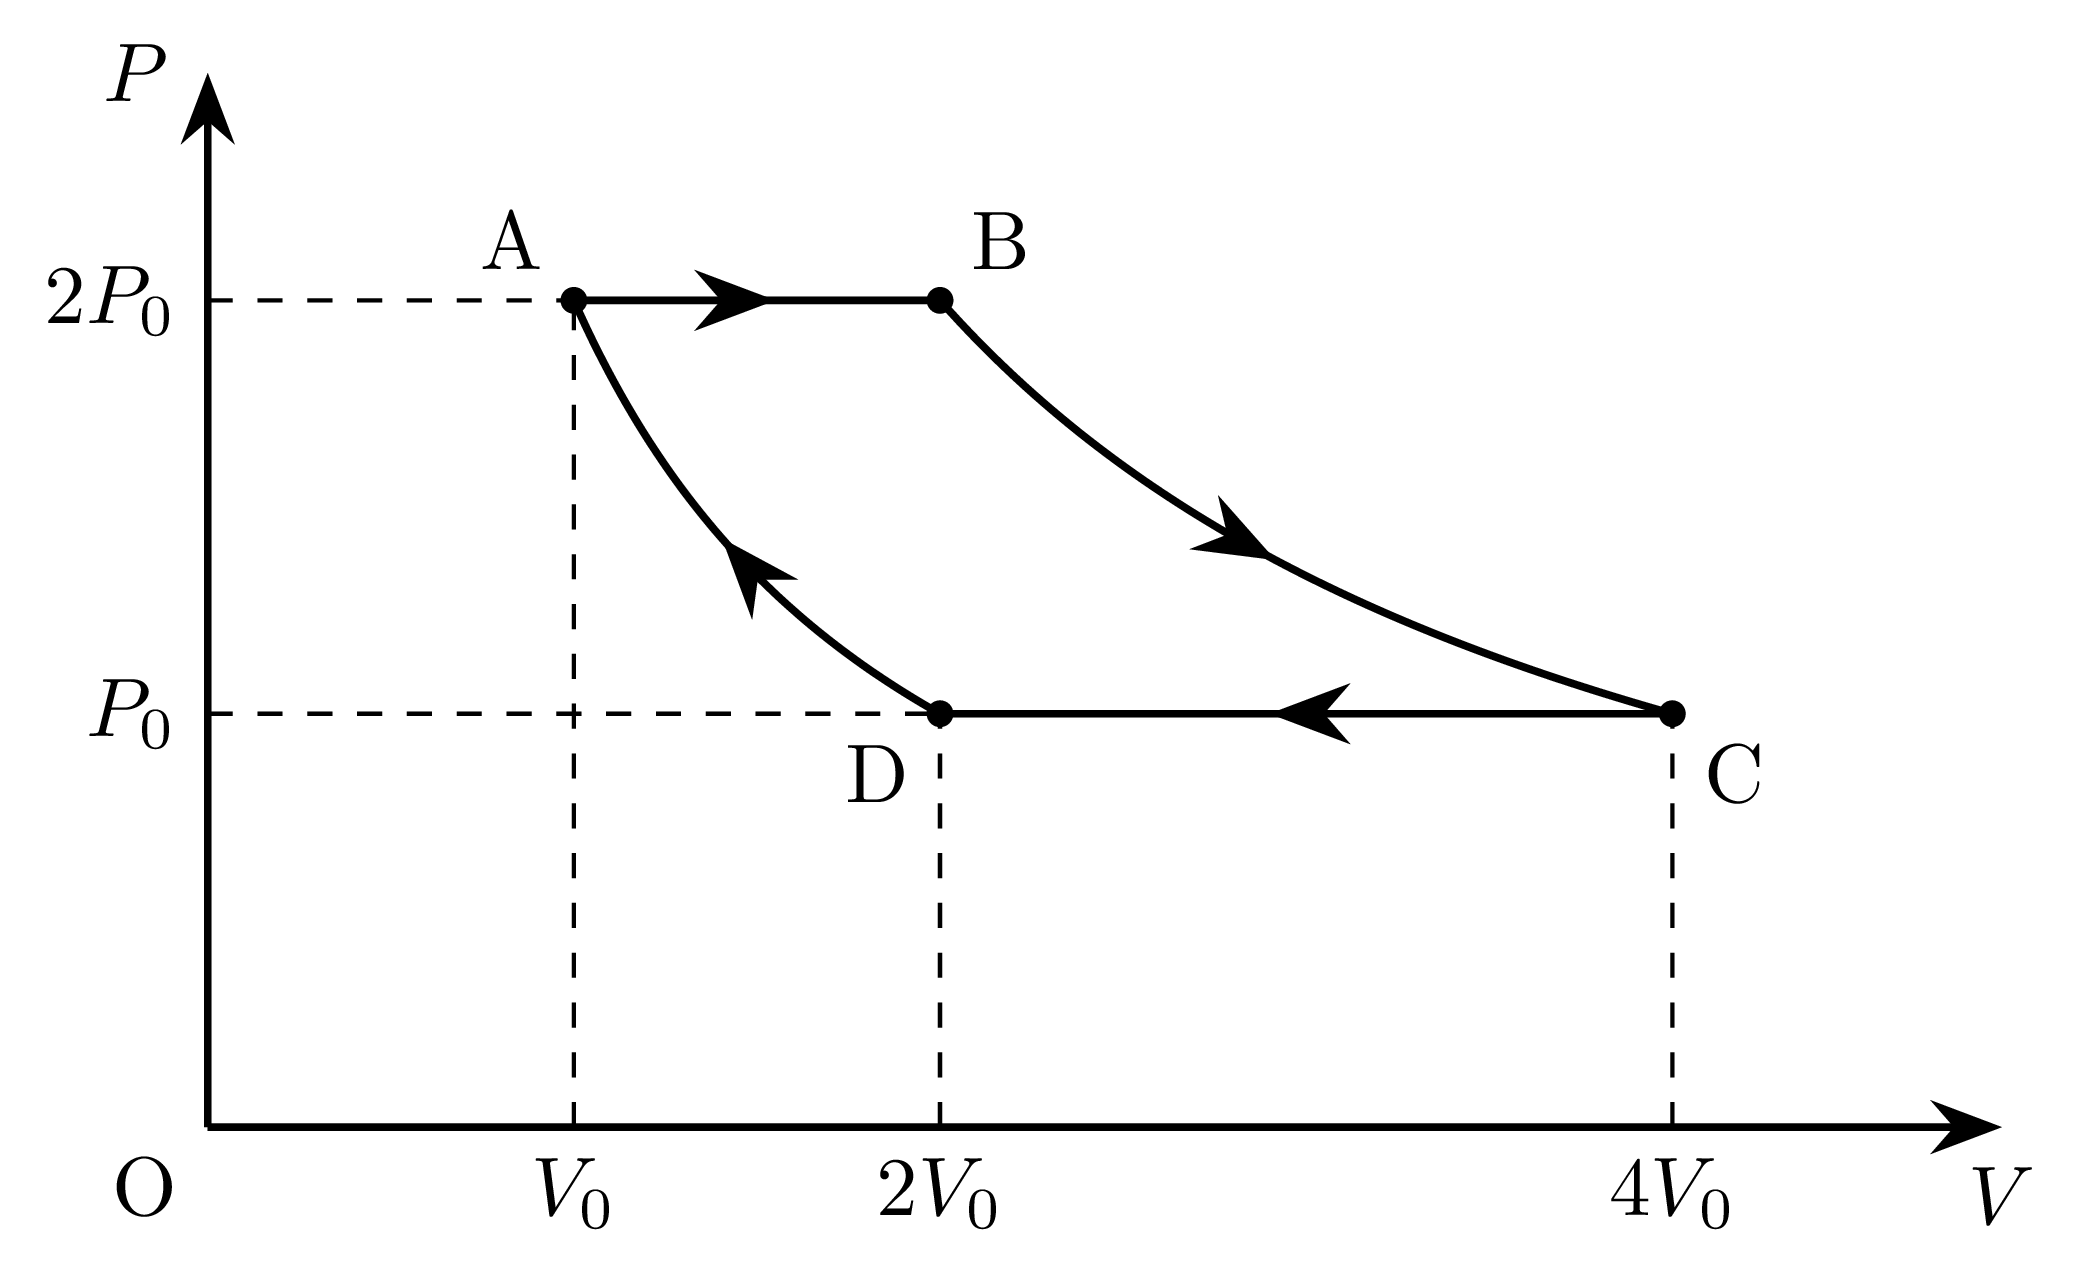
\includegraphics[keepaspectratio,width=76mm]{fig/ch15_ex7_pv.png}
\fi
\end{center}
\hspace*{\fill}\Ans
\end{kaitou}
